\documentclass{article}
\usepackage[english]{babel}
\usepackage[a4paper,top=2.54cm,bottom=2.54cm,left=2.54cm,right=2.54cm,marginparwidth=1.75cm]{geometry}
\usepackage{amsmath}
\usepackage{graphicx}
\usepackage{amsfonts}
\usepackage{amssymb}
\usepackage{enumerate}
\usepackage{enumitem}
\usepackage[colorlinks=true, allcolors=blue]{hyperref}
\usepackage{graphicx}
\usepackage[export]{adjustbox}
\usepackage{multirow}
\usepackage{mathtools}
\usepackage{MnSymbol}%
\usepackage{wasysym}%
\title{Calculus A(1): Homework 9}
\begin{document}
\maketitle
\section*{5.3.}
\subsection*{74.}
It would be nice if average values of integrable function obeyed the following rules on an interval $[a,b]$.
\begin{enumerate} [label=\textbf{\alph*.}]
    \item \[\mathrm{av}(f+g)=\mathrm{av}(f)+\mathrm{av}(g)\]
    \item \[\mathrm{av}(kf)=k\mathrm{av}(f),\forall k\in \mathbb{R}\]
    \item \[\mathrm{av}(f)\leq \mathrm{av}(g),(\forall x)(x\in[a,b]\rightarrow f(x)\leq g(x))\]
\end{enumerate}
Do these rules ever hold? Give reasons for your answers.
\subsection*{Solution.}
All of these rules hold.
\begin{enumerate}  [label=\textbf{\alph*.}]
    \item \[\mathrm{av}(f+g)=\frac{1}{b-a}\int _a^b(f(x)+g(x))dx=\frac{1}{b-a}\left(\int_a^b f(x)dx+\int_a^b g(x)dx\right)\]
    \[=\frac{1}{b-a}\int_a^b f(x)dx+\frac{1}{b-a}\int_a^b g(x)dx=\mathrm{av}(f)+\mathrm{av}(g)\blacksquare\]
    \item \[\mathrm{av}(kf)=\frac{1}{b-a}\int_a^b(kf(x))dx=k\cdot\frac{1}{b-a}\int_a^b f(x)dx=k\mathrm{av}(f)\blacksquare\]
    \item \[g(x)-f(x)\geq 0\Rightarrow \frac{1}{b-a}\int _a^b(g(x)-f(x))dx\geq 0\Rightarrow \mathrm{av}(g-f)\geq 0\Rightarrow \mathrm{av}(f)\leq \mathrm{av}(g)\blacksquare\]
\end{enumerate}
\subsection*{77.}
\textbf{Upper and lower sums for increasing functions}
\begin{enumerate} [label=\textbf{\alph*.}]
    \item Suppose the graph of a continuous function $f(x)$ rises steadily as $x$ moves from left to right across an interval $[a,b]$. Let $P$ be a partition of $[a,b]$ into $n$ subintervals of length $\Delta x=(b-a)/n$. Show by referring to the accompanying figure that the difference between the upper and lower sums for $f$ on this partition can be represented graphically as the area of a rectangle $R$ whose dimensions are $[f(b)-f(a)]$ by $\Delta x$. (\textit{Hint:} The difference $U-L$ is the sum of areas of rectangles whose diagonals $Q_0Q_1,Q_1Q_2,\dots,Q_{n-1}Q_n$ lie along the curve. There is no overlapping when these rectangles are shifted horizontally onto R.)
    \item Suppose that instead of being equal, the lengths $\Delta x_k$ of the subintervals of the partition $[a,b]$ vary in size. Show that 
    \[U-L \leq |f(b)-f(a)|\Delta x_{\mathrm{max}},\]
    where $\Delta x_{\mathrm{max}}$ is the norm of $P$,and hence that $\lim_{||P||\to 0}(U-L)=0$.
\end{enumerate}
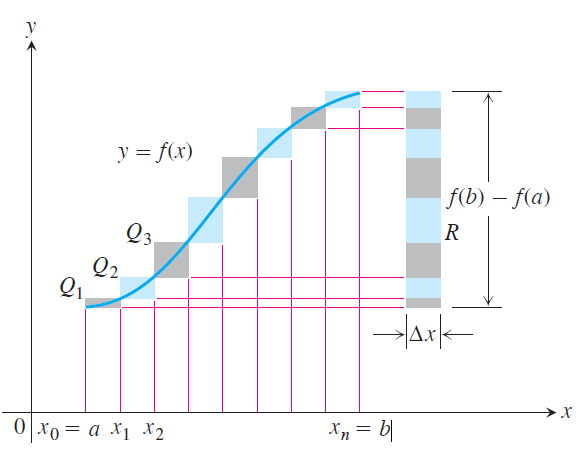
\includegraphics[scale=0.7]{img/20211218_calculusA_HW9_Fig_1.jpg}
\subsection*{Solution.}
\begin{enumerate} [label=\textbf{\alph*.}]
    \item With regards to each segment, its area is $(f(x_{i+1})-f(x_i))\cdot \Delta x$,
    so 
    \[U-L=\sum_{i=0}^{n-1} (f(x_{i+1})-f(x_i))\cdot \Delta x\]
    \[=(-f(x_0)+f(x_1)-f(x_1)+\cdots +f(x_n))\Delta x=(f(b)-f(a))\Delta x\]
    \item 
    \[U-L=\left\vert\sum_{i=0}^{n-1} (f(x_{i+1})-f(x_i))\cdot \Delta x_i\right|\leq\left|\sum_{i=0}^{n-1} (f(x_{i+1})-f(x_i))\right|\cdot \Delta x_{\mathrm{max}}=|(f(b)-f(a))|\Delta x_{\mathrm{max}}\]
    \[\lim_{||P||\to 0}(U-L)=\lim_{\Delta x_\mathrm{max}\to 0} |f(b)-f(a)|\Delta x_\mathrm{max}=0\]
\end{enumerate}
\subsection*{81.}
We say $f$ is \textbf{uniformly continuous} on $[a,b]$ if given any $\epsilon>0$ there is a $\delta>0$ such that if $x_1,x_2$ are in $[a,b]$ and $|x_1-x_2|<\delta$ then $|f(x_1)-f(x_2)|<\epsilon$. It can be shown that a continuous function on $[a,b]$ is uniformly continuous. Use this and the figure at the right to show that if $f$ is continuous and $\epsilon>0$ is given, it is possible to make $U-L\leq \epsilon\cdot(b-a)$ by making the largest of the $\Delta x_k$'s sufficiently small.\newline
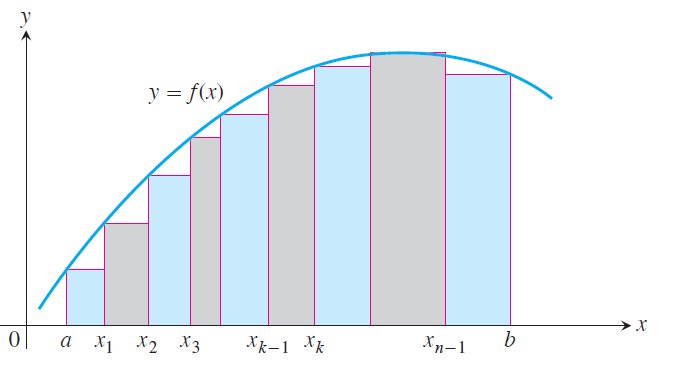
\includegraphics[scale=0.23]{img/20211218_calculusA_HW9_Figure_3a.png}
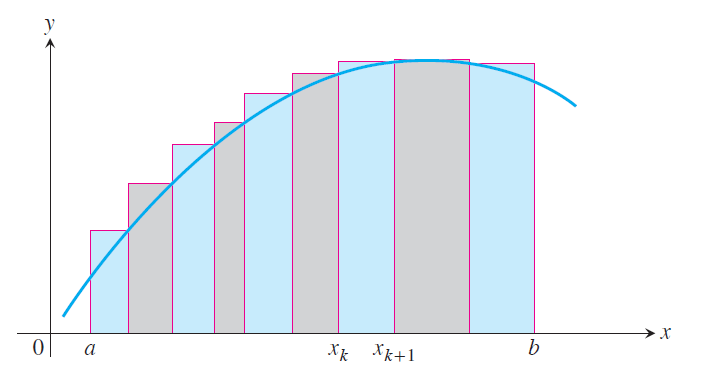
\includegraphics[scale=0.23]{img/20211218_calculusA_HW9_Figure_3b.png}
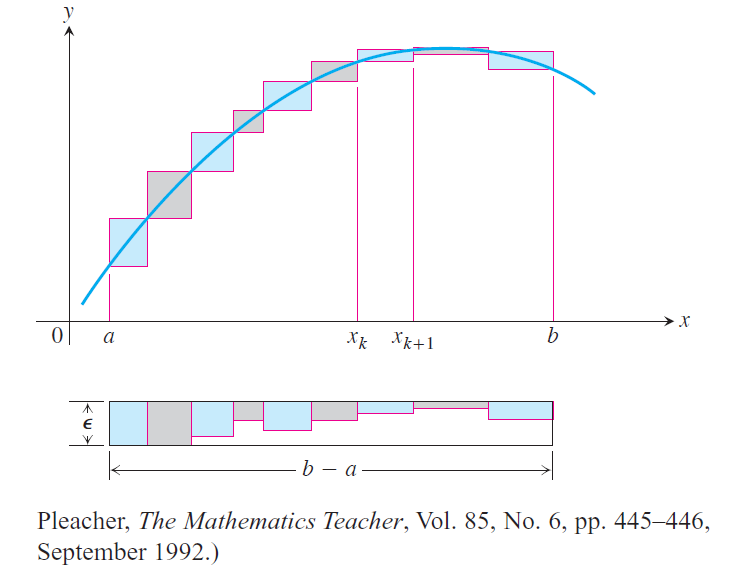
\includegraphics[scale=0.2]{img/20211218_calculusA_HW9_Figure_3c.png}
\subsection*{Solution.}
Let $x_{m_i},x_{M_i}\in [x_{i-1},x_i]$ such that 
\[(\forall x\in [x_{i-1},x_i])(f(x_{m_i})\leq f(x)\land f(x_{M_i})\geq f(x))\]
Then 
\[U-L=\sum_{i=1}^n(f(x_{M_i})-f(x_{m_i}))\Delta x_i.\]
$[a,b]$ is possible to be partitioned in a way that $\forall i\in\{1,2,\cdots,n\}, \Delta x_i<\delta$. That implies 
\[U-L=\sum_{i=1}^n(f(x_{M_i})-f(x_{m_i}))\Delta x_i<\sum_{i=1}^n\epsilon\cdot\Delta x_i=\epsilon\cdot (b-a)\]
\section*{5.4.}
\subsection*{68.}
Suppose that $f$ has a negative derivative for all values of $x$ and that $f(1)=0$. Which of the following statements must be true of the function
\[h(x)=\int_0^x f(t) dt?\]
Give reasons for your answers.
\begin{enumerate} [label=\textbf{\alph*.}]
    \item $h$ is a twice-differentiable function of $x$.
    \item $h$ and $dh/dx$ are both continuous.
    \item The graph of $h$ has a horizontal tangent at $x=1$.
    \item $h$ has a local maximum at $x=1$.
    \item $h$ has a local minimum at $x=1$.
    \item The graph of $h$ has an inflection point at $x=1$.
    \item The graph of $dh/dx$ crosses the $x$-axis at $x=1$.
\end{enumerate}
\subsection*{Solution.}
By definition, $h'(x)=f(x)$. Also,$\forall x\in \mathbb{R},f'(x)<0$, hence $h''$ exists and $\forall x\in \mathbb{R},h''(x)<0$ .\newline
$h'(1)=f(1)=0,$ and $h''(1)=f'(1)<0$, so $x=1$ is a maximum in some neighborhood of it, and has a horizontal tangent, and clearly it is not an inflection point. That means $h'$ changes sign when $x$ transverses the neighborhood of $x=1$. \newline
$h$ is twice-differentiable implies that its first derivative and its own  are both continuous. Therefore,\newline
\textbf{a.,b.,c.,d.,g.} are true, while \textbf{e.,f.} are false.
\section*{5.5.}
\subsection*{52.}
Evaluate the integral
\[\int \frac{\sin\sqrt{\theta}}{\sqrt{\theta\cos^3\sqrt{\theta}}}d\theta\]
\subsection*{Solution.}
\[\int\frac{\sin\sqrt{\theta}}{\sqrt{\theta\cos^3\sqrt{\theta}}}d\theta=4\int\left(\left(-\frac{1}{2}\cos^{-\frac{3}{2}}\sqrt{\theta}\right)(-\sin\sqrt{\theta})\left(\frac{1}{2\sqrt{\theta}}\right)\right)d\theta=\frac{4}{\sqrt{\cos\sqrt{\theta}}}+C, \]
where C is a constant.
\section*{5.6.}
\subsection*{78.}
Find the area of the region in the first quadrant bounded on the left by the $y-$axis, below by the curve $x=2\sqrt{y}$, above left by the curve $x=(y-1)^2$, and above right by the line $x=3-y$.\newline
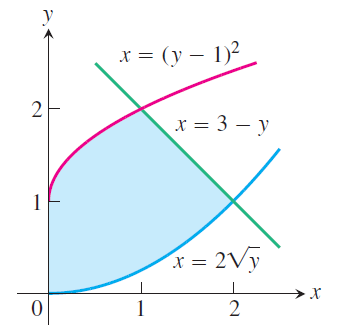
\includegraphics[scale=0.325]{img/20211218_calculusA_HW9_Fig_2.png}
\subsection*{Solution.}
Let $\Omega=\{(x,y)\in\mathbb{R}^2:x\geq (y-1)^2\land x\leq 3-y\land x\geq 0\land x\leq 2\sqrt{y}\}$.\newline
By inspection, (0,0),(2,1),(1,2) and (0,1) are the vertices of $\Omega$.
\[\iint_\Omega dxdy=\int_0^1 2\sqrt{y}dy+\int _1^2 (3-y-(y-1)^2)dy=\left.\frac{4}{3}y^{3/2}\right|_0^1+\left.\left(3y-\frac{1}{2}y^2-\frac{1}{3}(y-1)^3\right)\right|_1^2=\frac{5}{2}\]
\subsection*{87.}
If $f$ is a continuous function, find the value of the integral
\[I=\int _0^a \frac{f(x)dx}{f(x)+f(a-x)}\]
by making the substitution $u=a-x$ and adding the resulting integral to $I$.
\subsection*{Solution.}
\[I=\int_a^0\frac{f(a-u)}{f(a-u)+f(u)}(-du)=\int_0^a\frac{f(a-x)}{f(x)+f(a-x)}dx\]
So,
\[I=\frac{1}{2}\int_0^a\left(\frac{f(x)}{f(x)+f(a-x)}+\frac{f(a-x)}{f(x)+f(a-x)}\right)dx=\frac{1}{2}\int_0^a dx=\frac{1}{2}a\]
\section*{Additional and Advanced Exercises.}
\subsection*{8.}
Prove that 
\[\int_0^x\left(\int_0^uf(t)dt\right)du=\int_0^xf(u)(x-u)du\]
(\textit{Hint:} Express the integral on the right-hand side as the difference of two integrals. Then show that both sides of the equation have the same derivative with respect to $x$.)
\subsection*{Solution.}
Let $F(x)=\int_0^x f(t)dt$.\newline
By the fundamental theorem of Calculus,
\[F'(x)=\frac{d}{dx}\int_0^xf(t)dt=f(x),\]
So on one hand,
\[\int_0^x\left(\int_0^uf(t)dt\right)du=\int_0^x F(u)du.\]
On the other hand,
\[\int_0^xf(u)(x-u)du=F(u)(x-u)|_0^x-\int_0^x F(u)(-1)du=\int_0^x F(u)du\]
Hence,
\[\int_0^x\left(\int_0^uf(t)dt\right)du=\int_0^x F(u)du=\int_0^xf(u)(x-u)du\blacksquare\]
\section*{Bonus.}
\subsection*{1.}
Show that if $f:[a,b]\to\mathbb{R}$ is continuous, then $f$ is uniformly continuous.
\subsection*{Solution.}
Fix the $\epsilon>0$ given.\newline
By continuity of $f$ on $[a,b]$, let $U_x$ be a set such that it is the $\frac{\delta_x}{2}$-neighborhood of $x$ for $x\in[a,b]$, i.e.
\[U_x=\left\{y:|x-y|<\frac{\delta_x}{2}\right\}\]
satisfying the property that if $x_0\in U_x$, then 
\[|f(x)-f(x_0)|<\epsilon/2\]
With this definition, we can see that
\[[a,b]\subset \bigcup_{x\in[a,b]}U_x\]
As $[a,b]$ is compact (closed and bounded), then there is a finite number of $x_i\in[a,b]$ that the union of their neighborhood contains $[a,b]$.
\[[a,b]\subset \bigcup_{i=1}^n U_{x_i}\]
Pick $\delta$ as the smallest of $\frac{1}{2}\delta_{x_i}$.\newline
Then, $\forall x,y\in[a,b]$, $x\in U_{x_i}$ for some $i$.  If given that $|x-y|<\delta$, then
\[|x_i-y|\leq |x_i-x|+|x-y|<\frac{1}{2}\delta_{x_i}+\delta\leq \delta_{x_i}\]
So $|x-x_i|<\delta_{x_i}$, $|y-x_i|<\delta_{x_i}$.
As $f$ is continuous on $[a,b]$, the above implies that 
\[|f(x)-f(y)|\leq |f(x)-f(x_i)|+|f(y)-f(x_i)|<\frac{\epsilon}{2}+\frac{\epsilon}{2}=\epsilon\blacksquare \]

\end{document}